\chapter{Technologien}

%
% TypeScript
%
\section{TypeScript}
\label{sec:typescript}

TypeScript ist eine Programmiersprache von Microsoft, die JavaScript um ein Typensystem erweitert. So können u.A. Fehler frühzeitig (während der Entwicklung) erkannt und behoben sowie Autovervollständigungen geboten werden. TypeScript-Code kann nicht direkt ausgeführt werden, sondern muss vorher zu JavaScript transpiliert werden. Jeder gültige JavaScript-Code ist dadurch auch gültiger TypeScript-Code \cites[vgl.][]{TypeScript}[vgl.][]{TypeScriptForJSDevelopers}.

Abbildung \ref{fig:typescript} zeigt einen TypeScript-Code, bei dem der Parameter der Funktion als Array typisiert wurde. Wird nun z.B. eine ungültige Methode, wie \lstinline{trim} aufgerufen, gibt TypeScript eine Fehlermeldung aus, da Arrays diese Methode nicht besitzen.

\begin{figure}[H]
  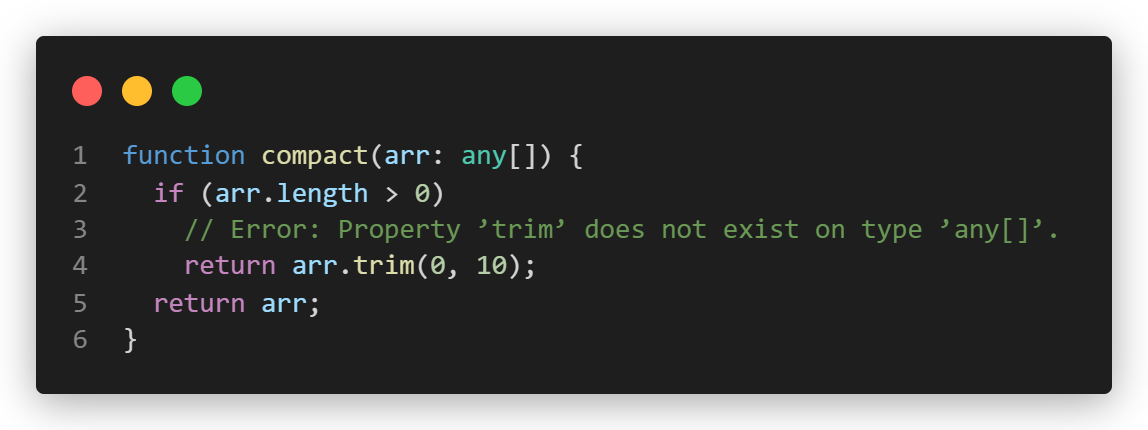
\includegraphics[width=0.9\textwidth]{images/typescript-example.png}
  \centering
  \caption[Beispiel für TypeScript-Code]{Beispiel für TypeScript-Code}
  \label{fig:typescript}
\end{figure}

Bestehende JavaScript-Projekte können inkrementell auf TypeScript umgestellt werden, indem TypeScript vorerst nur als Typ-Überprüfung verwendet wird. Dabei können Kommentare in den vorhandenen JavaScript-Code eingefügt werden, wodurch TypeScript anschließend den Code überprüfen kann (siehe Abildung \ref{fig:typescript-js}) \cite[vgl.][]{TypeScript}. Da hierbei anders als in Abbildung \ref{fig:typescript} kein TypeScript-Code eingefügt wird, muss der Code nicht transpiliert werden, bietet jedoch auch nicht den vollen Funktionsumfang von TypeScript.

\begin{figure}[H]
  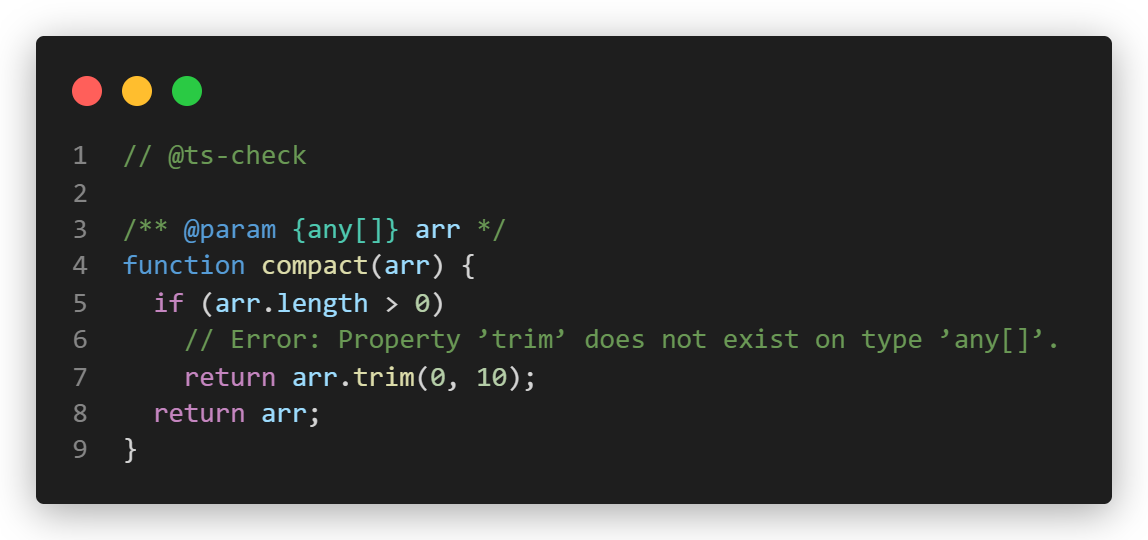
\includegraphics[width=0.9\textwidth]{images/typescript-example-js.png}
  \centering
  \caption[Erweiterung von JavaScript-Code um TypeScript Typ-Überprüfung]{Erweiterung von JavaScript-Code um TypeScript Typ-Überprüfung}
  \label{fig:typescript-js}
\end{figure}

%
% Sass
%
\section{Sass}
\label{sec:sass}
Sass ist eine Stylesheet-Sprache, die zu CSS kompiliert wird. Sie vereinfacht die Verwendung von CSS, indem weitere Funktionen, wie z.B. Verschachtlung, bereitgestellt werden. Dabei ist sie vollständig zu CSS kompatibel, d.h. jeder CSS-Code ist gültiger Sass-Code \cite[vgl.][]{SassDocs}. Die erweiterten Funktionen helfen dabei robusten und wartbaren CSS-Code zu schreiben \cite[vgl.][]{SassDocs}.

Abbildung \ref{fig:store-definition} zeigt einen Vergleich desselben Codes in CSS und Sass. Durch Sass kann hierbei redundanter Code verhindert werden. Für Interessierte sei für weitere Funktionen auf \cite{SassGuide} verwiesen.

\begin{figure}[!htb]
  \begin{minipage}{0.48\textwidth}
    \centering
    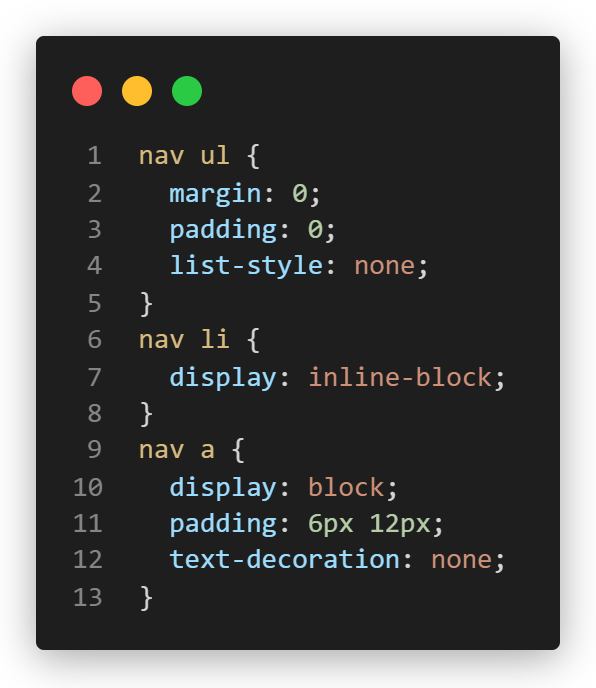
\includegraphics[width=.95\linewidth]{images/css-example.png}
  \end{minipage}\hfill
  \begin{minipage}{0.48\textwidth}
    \centering
    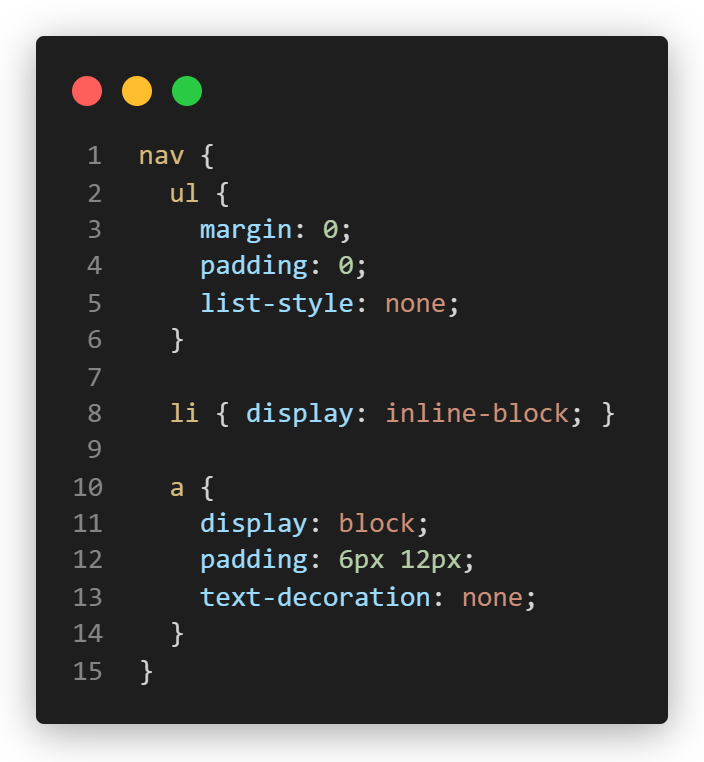
\includegraphics[width=1\linewidth]{images/sass-example.png}
  \end{minipage}
  \caption[Vergleich von CSS und Sass]{Vergleich von CSS (links) und Sass (rechts) am Beispiel von Verschachtlung \cite{SassGuide}}
  \label{fig:store-definition}
\end{figure}

%
% Bootstrap
%
\section{Bootstrap}
Um die Gestaltung der Benutzeroberfläche (siehe Kapitel \ref{sec:struktur-frontend}) zu vereinfachen, wird Bootstrap verwendet. Bootstrap ist Werkzeugsatz, der u.A. vorgefertigte Komponenten bzw. CSS sowie Icons bereitstellt \cite[vgl.][]{Bootstrap}.

%
% Vue
%
\section{Vue}

Für die Erstellung der Benutzeroberfläche (im Folgenden \glqq Frontend\grqq{} genannt) wird Vue (Version 3.2) verwendet. Vue ist ein progressives JavaScript-Framework, das die Frontend-Entwicklung vereinfachen soll. Progressiv bedeutet hierbei, das es für das gesamte Frontend oder auch nur für Teile dessen verwendet werden kann. Vue kann folglich mit anderen Technologien verwendet oder Schritt-für-Schritt (progressiv) in bereits vorhandene Projekte integriert werden \cite[vgl.][]{VueIntroduction}.

%
% Vue - Grundlagen von Komponenten
%
\subsection{Grundlagen von Komponenten}
\begin{figure}[H]
  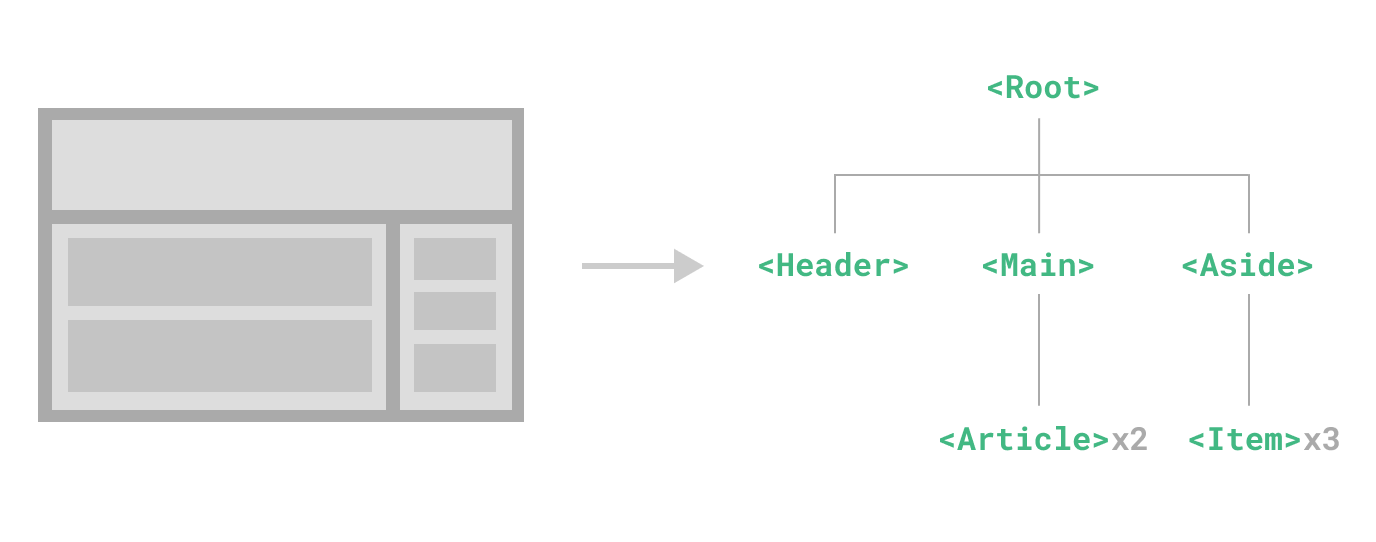
\includegraphics[width=0.9\textwidth]{images/vue-components.png}
  \centering
  \caption[Vue-Komponenten]{Strukturierung des Frontends durch Vue-Komponenten \cite{VueComponentBasics}}
  \label{fig:vue-components}
\end{figure}

Vue-Komponenten erlauben die Unterteilung des Frontends in unabhängige, isolierte und wiederverwendbare Teile. So wird das Frontend in kleinere Komponenten gegliedert (siehe Abbildung \ref{fig:vue-components}), die dann die benötigte Logik kapseln und unabhängig entwickelt werden können \cite[vgl.][]{VueComponentBasics}.

Vue bietet mehrere Möglichkeiten, um eine Komponente zu definieren. Im Rahmen dieser Studienarbeit werden sogenannte \aclu{SFC} (\acs{SFC}) verwendet (siehe Abbildung \ref{fig:vue-example}). Jede Komponente wird hierbei in einer Datei mit der Dateiendung \lstinline{.vue} definiert. Nachdem die Komponente in einer anderen Datei importiert wurde, kann sie wie ein herkömmliches HTML-Element verwendet werden (siehe Abbildung \ref{fig:vue-example-usage}) \cite[vgl.][]{VueComponentBasics}.

\begin{figure}[!htb]
  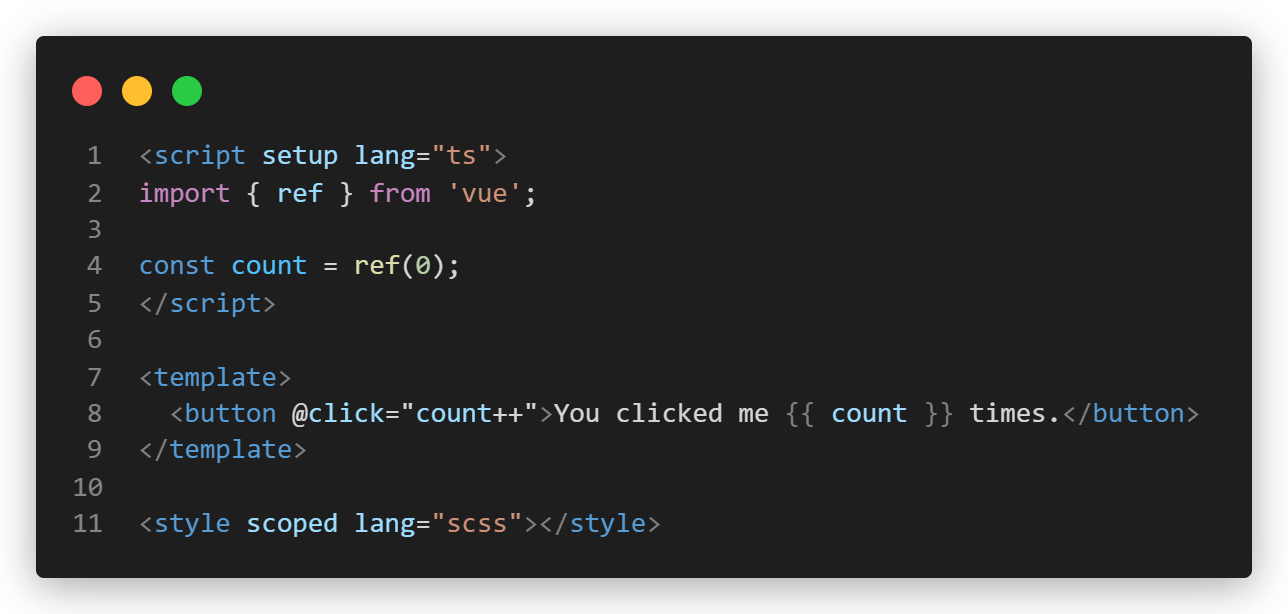
\includegraphics[width=0.9\textwidth]{images/vue-example.png}
  \centering
  \caption[Beispiel einer Vue-Komponente]{Beispiel einer Vue \ac{SFC} \cite{VueComponentBasics}}
  \label{fig:vue-example}
\end{figure}

\begin{figure}[!htb]
  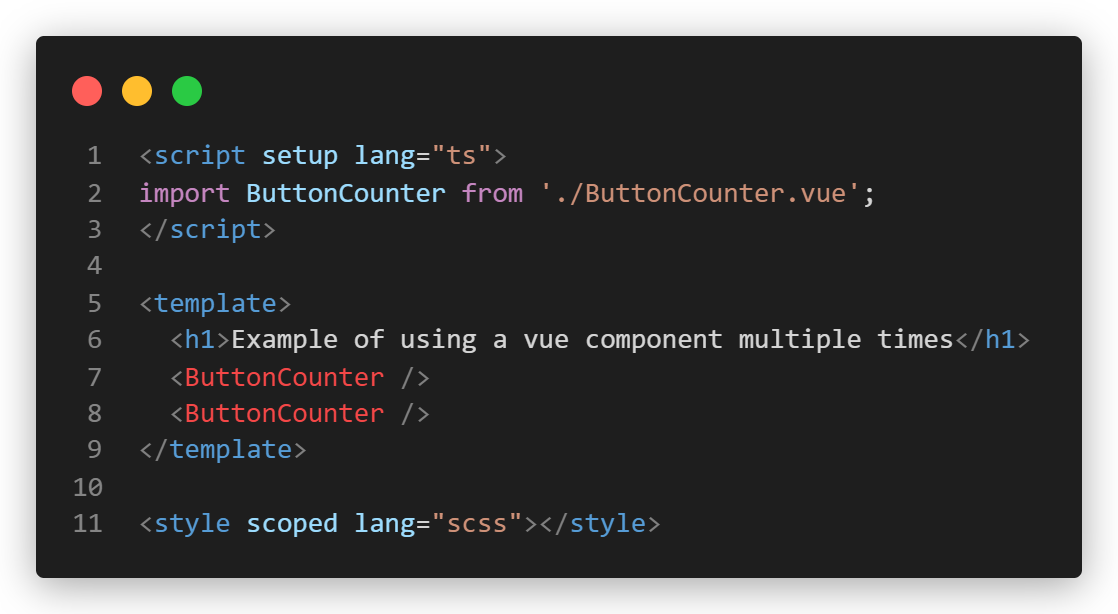
\includegraphics[width=0.9\textwidth]{images/vue-example-usage.png}
  \centering
  \caption[Verwendung einer Vue-Komponente]{Verwendung einer Vue \ac{SFC} \cites[vgl.][]{VueComponentBasics}[vgl.][]{VueSFC}}
  \label{fig:vue-example-usage}
\end{figure}

\textbf{Sprach-Blöcke} \\
In \acp{SFC} können standardmäßig die drei Sprach-Blöcke \lstinline{<template>} (HTML), \lstinline{<script>} (JavaScript) und \lstinline{<style>} (CSS) verwendet werden (siehe Abbildung \ref{fig:vue-example}), die den entsprechenden Code der Komponente beinhalten. Mit dem \lstinline{scoped}-Attribut des \lstinline{<style>}-Blocks kann das CSS für die Komponente gekapselt werden, d.h. es wird nur innerhalb der Komponente angewendet \cite[vgl.][]{VueSFC}.

\textbf{TypeScript und Sass} \\
Für die Entwicklung des Frontends sollen TypeScript (Version 4.4) und Sass (Version 1.43) verwendet werden, die bereits in Kapitel \ref{sec:typescript} und \ref{sec:sass} erläutert wurden. So soll sichergestellt werden, dass Fehler bereits während der Entwicklung behoben werden können und ein robustes, wartbares Frontend entsteht.

Um TypeScript in einer \ac{SFC} verwenden zu können, muss der \lstinline{<script>}-Block (siehe Abbildung \ref{fig:vue-example}) um das Attribut \lstinline{lang="ts"} erweitert werden. Sass kann nach der Erweiterung des \lstinline{<style>}-Blocks um das Attribut \lstinline{lang="scss"} verwendet werden \cite[vgl.][]{VueSFC}.

%
% Vue - Composition API
%
\subsection{Composition API}
Vue-Komponenten können (innerhalb des \lstinline{<script>}-Blocks) entweder mit Vue's Options API oder mit der Composition API erstellt werden. Aufgrund der Empfehlung von Vue wird im Rahmen dieser Studienarbeit die Composition API in Verbindung mit \acp{SFC} verwendet. Des Weiteren wird das \lstinline{setup}-Attribut des \lstinline{<script>}-Blocks ergänzt (siehe Abbildung \ref{fig:vue-example}), wodurch der Umgang mit der Composition API erleichtert wird. Unter Anderem werden alle Imports sowie Variablen für den \lstinline{<template>}-Block bereitgestellt \cite[vgl.][]{VueIntroduction}.

In Abbildung \ref{fig:vue-example} wird bereits die Composition API verwendet. Im Vergleich dazu zeigt Abbildung \ref{fig:vue-example-options-api} dieselbe Komponente unter Verwendung der Options API.

\begin{figure}[!htb]
  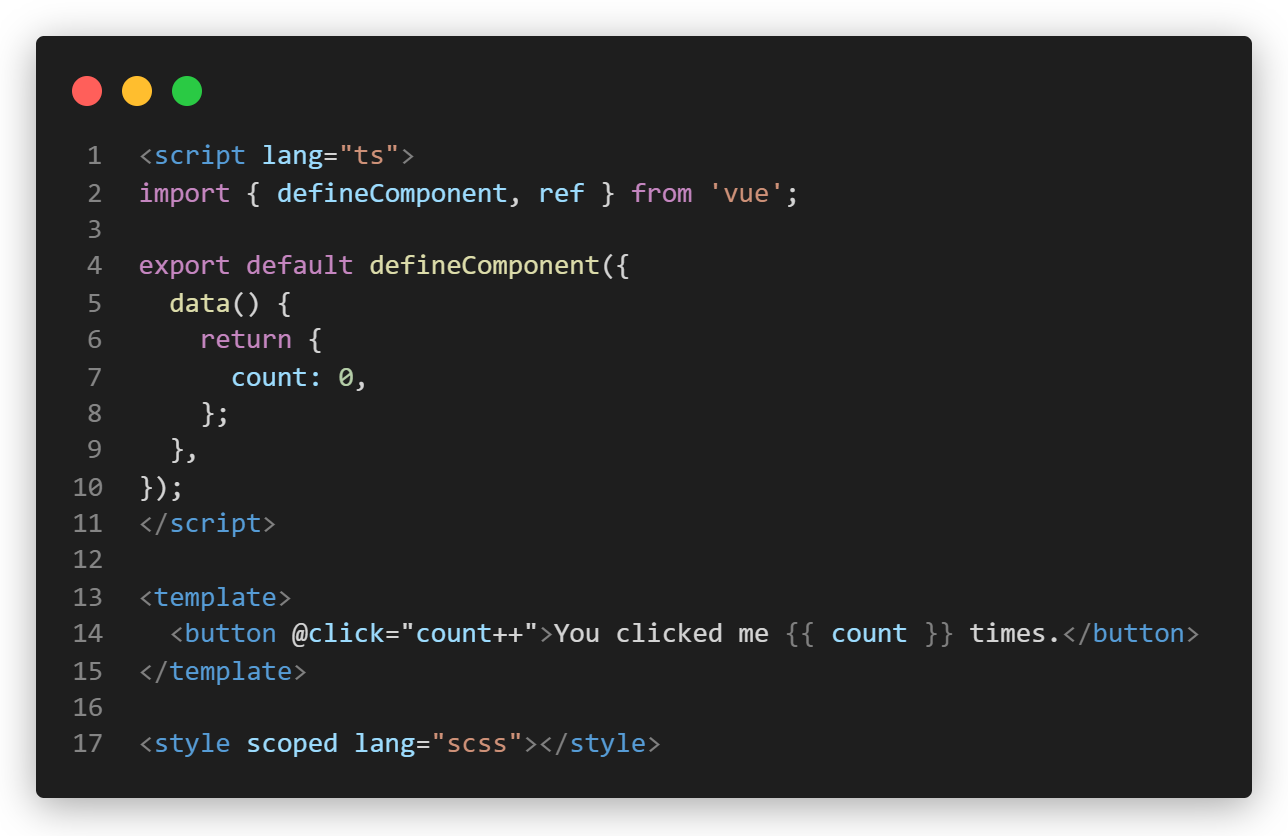
\includegraphics[width=0.9\textwidth]{images/vue-example-options-api.png}
  \centering
  \caption[Beispiel einer Vue-Komponente mit Options API]{Beispiel einer Vue-Komponente mit Options API \cites[vgl.][]{VueIntroduction}[vgl.][]{VueSFC}}
  \label{fig:vue-example-options-api}
\end{figure}

%
% Vue - Reaktivität
%
\subsection{Reaktivität}
Vue stellt mehrere Funktionen zum Erstellen von reaktiven Variablen bereit. In Abbildung \ref{fig:vue-example} wurde bereits die Funktion \lstinline{ref} verwendet, die einen Wert reaktiv macht \cite[vgl.][]{VueApiReactiveCore}. Wird ein reaktiver Wert z.B. im \lstinline{<template>}-Block der Komponente verwendet, aktualisiert Vue automatisch den HTML-Code, wenn sich der Wert ändert \cite[vgl.][]{VueReactiveFundamentals}. Würde man also in Abbildung \ref{fig:vue-example} \glqq \lstinline{const count = ref(0)}\grqq{} durch \glqq \lstinline{const count = 0}\grqq{} ersetzen, würde im HTML-Code selbst bei einer Änderungen des Wertes immer \glqq \lstinline{You clicked me 0 times.}\grqq{} angezeigt werden, da \lstinline{count} dann nicht mehr reaktiv ist.

Für weitere Funktionen bezüglich der Reaktivität sei für Interessierte auf \cite{VueApiReactiveCore} verwiesen. Für detaillierte Informationen über Vue empfiehlt sich die offizielle Dokumentation, die unter \cite{VueIntroduction} zu finden ist.

%
% Strapi CMS
%
\section{Strapi CMS}
Strapi ist ein sogenanntes headless \ac{CMS}, d.h. es ist eine Software zum Verwalten von Inhalten und Daten. Headless bedeutet hierbei, dass das \ac{CMS} ausschließlich die Verwaltung (Erstellung, Speicherung etc.) der Inhalte übernimmt und sie nicht in z.B. einer Webanwendung oder App darstellt. Traditionelle \ac{CMS}, wie z.B. WordPress, bündeln im Vergleich dazu die Verwaltung der Inhalte und die Darstellung in derselben Anwendung \cite[vgl.][]{StrapiHeadlesssCMS}.

Strapi ist in JavaScript geschrieben, Open Source und kann vollständig angepasst werden. Es soll die Entwicklung von APIs deutlich vereinfachen und kann selber gehostet werden. Dazu wird eine Benutzeroberfläche bereitgestellt, über die Inhaltstypen erstellt und verwaltet werden können. Anschließend sind diese durch REST oder GraphQL Endpunkte zugänglich \cite[vgl.][]{Strapi}.

Im Rahmen dieser Studienarbeit wird Strapi (Version 4.x) als API (im Folgenden \glqq Backend\grqq{} genannt) verwendet, um Blogbeiträge zu verwalten. Eine detaillierte Betrachtung des CMS erfolgt in Kapitel \ref{sec:struktur-backend}.
